\documentclass{beamer}

\usepackage{verbatim}

\usetheme{CambridgeUS}

\usecolortheme{dolphin}

% De kleur van de url links bepalen
\definecolor{links}{HTML}{FF4444}
\hypersetup{colorlinks,linkcolor=,urlcolor=links}

%\setbeamertemplate{footline}[page number]

\setbeamertemplate{navigation symbols}{}

\title{Servlets en JSP}
\subtitle{deel \'e\'en}
\author{Java Cursisten}
\institute{INTEC Brussel}
\date{\today}

\begin{document}

\begin{frame}

\titlepage

\end{frame}


\begin{frame}

\frametitle{Overzicht}
\tableofcontents

\end{frame}


\section{Van web site naar web app}


\begin{frame}

\frametitle{Swing and console are going out!}

{\LARGE We gaan web apps bouwen.\\~\\

Hiervoor moeten we eerst Servlets en JSP leren.\\~\\

Hiermee kunnen we dynamische, interactieve web sites maken ipv statische (HTML only) websites.}

\end{frame}


\section{World Wide Web}


\begin{frame}

\frametitle{World Wide Web}

\begin{figure}

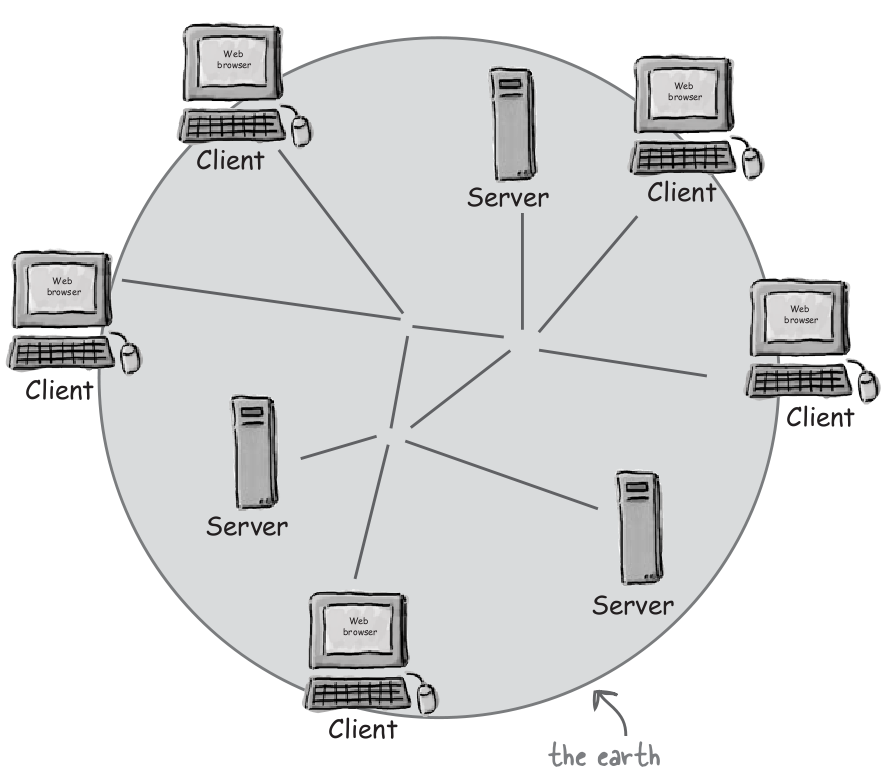
\includegraphics[width=220pt]{FigureOne.png}

\end{figure}

\end{frame}


\begin{frame}

\frametitle{Wat doet een web server}

{\Large \begin{enumerate}
  \item Een gebruiker vraagt een \textit{resource} aan een web \textit{server} met zijn web \textit{browser}
  \item De web server ontvangt de vraag (\textit{request}) en stuurt de gebruiker iets terug.
\end{enumerate}

De resource die de web server terugstuurt kan een HTML pagina zijn, een foto, een video, een PDF,...\\
Kortweg : \textbf{de client vraagt iets en de server geeft iets}}

\end{frame}


\begin{frame}

\frametitle{\textbf{Tenzij...}}

{\Large de client een request doet naar een resource die de server niet kan vinden\\~\\
Dan krijg je een (bekende) foutmelding :\\~\\}

\begin{center}
{\huge \textbf{{404 Not Found}}}\\~\\
\end{center}

{\Large Dit is \'e\'en van de vele \href{https://en.wikipedia.org/wiki/List_of_HTTP_status_codes}{HTTP status codes}.}

\end{frame}


\begin{frame}

\begin{figure}

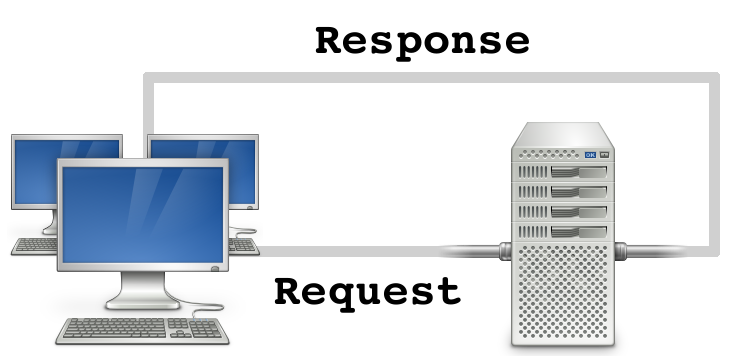
\includegraphics[width=300pt]{ClientsAndServers.png}

\end{figure}

\end{frame}


\begin{frame}

\frametitle{SERVER}

{\LARGE Als we het woord 'server' gebruiken kunnen we het hebben over de \textbf{fysieke machine} {\huge \textbf{\textit{of}}} over de web server \textbf{applicatie} (software).\\~\\
Enkel als het onderscheid belangrijk is zullen we duidelijk specifi\"eren of het over de machine of de software gaat.}

\end{frame}


\begin{frame}

\frametitle{CLIENT}

{\LARGE Als we het woord 'client' gebruiken kunnen we het hebben over de \textbf{fysieke persoon} {\huge \textbf{of}} over de browser \textbf{applicatie}.\\~\\
Het onderscheid hiertussen is veelal onbelangrijk voor ons dus voor ons geldt : \textbf{de client is de browser app die doet wat de gebruiker vraagt}.}

\end{frame}


\begin{frame}

\frametitle{OVERZICHT}

{\Large \begin{enumerate}
  \item Gebruiker klikt op een link naar een html pagina in de browser
  \item Browser maakt een request en stuurt dit naar de server
  \item Server zoekt de gevraagde html pagina
  \item Server maakt een response en stuurt dit naar de browser
  \item Browser krijgt de gevraagde html pagina en 'renders it'
  \item Gebruiker ziet de nieuwe pagina op het scherm (en vindt dit de normaalste zaak van de wereld)
\end{enumerate}}

\end{frame}


\begin{frame}

\frametitle{(HTML) en HTTP}

{\Large HTTP is het protocol (i.e. een serie afspraken) waardoor servers en clients met elkaar kunnen communiceren met HTTP requests
en HTTP responses.}\\~\\

{\huge HyperText Transfer Protocol}\\~\\

\end{frame}


\begin{frame}

\frametitle{De lagen van het internet}

{\Large \begin{enumerate}
  \item Link layer biedt communicatie technologie voor lokale netwerken (bv. Ethernet)
  \item Internet layer connecteert lokale netwerken \\(bv. IP : Internet Protocol)
  \item Transport layer biedt host-to-host communicatie \\(bv. TCP : Transport Communication Protocol)
  \item Application layer biedt process-to-process communicatie (bv. HTTP voor communicatie tussen web clients en web servers)
\end{enumerate}}

\end{frame}


\begin{frame}

\begin{center}
{\Huge VIDEO}
\end{center}

\end{frame}


\begin{frame}

\frametitle{HTTP response bevat}

{\LARGE \begin{itemize}
  \item een header met \href{https://en.wikipedia.org/wiki/List_of_HTTP_header_fields}{header fields} \\met metadata van de response.
  \item een body met de eigenlijke data \\(bv. html pagina)
\end{itemize}}

\end{frame}


\begin{frame}

\frametitle{HTTP request bevat}

{\Large een method name (of de soort request)\\~\\

GET is de simpelste HTTP methode en vraagt naar een resource\\~\\
POST is een krachtigere HTTP methode waarmee je een resource kan vragen en tegelijk form data naar de server kan sturen.\\~\\
Er zijn er meer maar die gaan wij niet gebruiken}

\end{frame}


\begin{frame}

\frametitle{GET requests kunnen toch ook data versturen ?}

{\Large Technisch gezien wel maar er zijn wel verschillen...

\begin{enumerate}
  \item De maximale hoeveelheid characters is relatief beperkt
  \item De data die je verstuurt met een GET request wordt toegevoegd aan de URL (niet echt veilig)
  \item Een GET Request kan gebookmarked worden en een POST Request niet
\end{enumerate}}

\end{frame}


\begin{frame}

\frametitle{Oefening : GET of POST ?}

{\large \begin{itemize}
\item Een gebruiker stuurt een login en paswoord.
\item Een gebruiker vraagt een nieuwe pagina via een hyperlink.
\item Een chatter stuurt een geschreven boodschap.
\item Een gebruiker drukt op een 'next' knop \\om de volgende pagine te laden.
\item Een gebruiker drukt op een 'log out' \\knop op een online banking site.
\item Een gebruiker drukt op de 'back' knop van zijn browser.
\item Een gebruiker stuurt een naam en adres form naar de server.
\item Een gebruiker maakt een radio button selectie.
\end{itemize}}

\end{frame}


\begin{frame}

\frametitle{URL}

{\LARGE URL : \textbf{u}niform \textbf{r}esource \textbf{l}ocator\\~\\}

{\Large \url{http://www.duckduckgo.com:80/lite?q=URL}}\\~\\

\begin{itemize}
  \item http : dit is het protocol
  \item www.duckduckgo.com : dit is de server
  \item 80 : TCP poort (optioneel)
  \item lite : path
  \item ?q=URL : query string (optioneel)
\end{itemize}

\end{frame}


\begin{frame}

\frametitle{TCP port}

{\Large Dit is gewoon een nummer.\\

16 bits die een specifiek software programma aangeven op de computer\\

Voorbeelden :

\begin{itemize}
  \item HTTP : 80
  \item HTTPS : 443
  \item SMTP : 25
  \item POP3 : 110
  \item FTP : 21
\end{itemize}}

16 bits dus 65536 mogelijkheden (0 tot 65535)\\
poorten van 0 tot 1023 zijn voorbehouden voor \href{https://en.wikipedia.org/wiki/List_of_TCP_and_UDP_port_numbers\#Well-known_ports}{bekende services}

\end{frame}

\section{STATIC vs DYNAMIC}


\begin{frame}

\frametitle{STATIC}

{\Large Een gewone web server kan zeer goed overweg met statische web pagina's.\\~\\
Op de server staan gewoon een hoop bestanden die de client kan opvragen.\\~\\
Elke gebruiker ziet dus net hetzelfde als elke andere gebruiker.\\~\\
Een statische web site heeft twee beperkingen.}

\end{frame}


\begin{frame}

\frametitle{eesrte beperking}

{\Large Zo een server kan geen dynamische content produceren.\\~\\
Just-in-time pagina's zijn dynamisch gecre\"erde pagina's die
voor de request nog niet bestonden.\\~\\Deze pagina's worden gegenereerd
door een 'helper' applicatie.\\~\\ De web server stuurt dan de JIT html pagina
mee met de response naar de gebruiker.}

\end{frame}


\begin{frame}

\frametitle{tweede beperking}

{\Large Een gewone web server kan geen data opslaan.\\~\\Een gewone web server
is dus non-persistent. \\~\\Hiervoor heeft een web server ook een 'helper'
applicatie nodig die dit voor zijn rekening neemt.}

\end{frame}


\begin{frame}

\frametitle{SERVLET}
{\Large 
De beruchte 'helper' applicaties die een web server nodig heeft om de
twee voornoemde beperkingen te overwinnen zijn...}\\~\\

\begin{center}
\textbf{}{\Huge SERVELTS!}\\
{\tiny(in de Java-wereld)}
\end{center}

\end{frame}


\begin{frame}

\frametitle{Apache Tomcat}

\begin{figure}


\includegraphics[width=170pt]{Tomcat-logo.png}

\end{figure}

\begin{center}
{\LARGE \href{http://tomcat.apache.org/}{Onze web server en servlet container}}
\end{center}

\end{frame}


\begin{frame}

\frametitle{Deployment Descriptor (web.xml)}

{\Large Dit is een configuratie bestand van Tomcat\\~\\

Hierin kun je Servlets registreren en linken aan URL's\\~\\

Zoals je aan de extensie kan zien is dit een XML bestand\\(hierover later meer)}

\end{frame}


\section{Zelf proberen!}


\begin{frame}

\frametitle{installing Tomcat}

{\LARGE Download Tomcat : \\{\Large \url{http://tomcat.apache.org/download-70.cgi}}\\~\\

Installeer Tomcat : \\unzippen in de folder waar je de server wilt hebben staan\\~\\

Done.}

\end{frame}


\begin{frame} 

\frametitle{Dynamic Web Page maken}

{\Large \begin{enumerate}
  \item File - New - Dynamic Web Project
  \item Bij Project name 'Eerste Dynamische Website' tikken
  \item Plaats een vinkje bij 'Generate web.xml'
  \item Finish!
\end{enumerate}}

\end{frame}


\begin{frame}

\frametitle{statische pagina toevoegen}

{\Large \begin{enumerate}
  \item Rechtermuisknop op WebContent : New - HTML file
  \item Tik 'Welkom' bij File name
  \item De tekst van de volgende slide ingeven
\end{enumerate}}

\end{frame}


\begin{frame}[fragile]

\begin{verbatim}

<!doctype html>
<html lang="nl">
  <head>
    <meta charset="UTF-8">
    <title>Welkom bij mijn eerste dynamische website</title>
    <link rel="stylesheet" href="styles/default.css" />
  </head>
  <body>
    <h1>Welkom bij mijn eerste dynamische website</h1>
    <img src="images/Tomcat-logo.png" alt="Tomcat"/>
  </body>
</html>


\end{verbatim}

\end{frame}


\begin{frame}

\frametitle{een afbeelding toevoegen}

\begin{enumerate}
  \item Rechtermuisknop op WebContent : New - Folder
  \item Tik 'Images' bij name en kies Finish
  \item Rechtermuisknop op images : Import - General - File System en druk op Next
  \item Navigeer naar Tomcat-logo.png (bij het .tex bestand van deze slideshow), vink het aan en druk op Finish
\end{enumerate}

\end{frame}


\begin{frame}[fragile]

\frametitle{een CSS toevoegen}

\begin{enumerate}
  \item Rechtermuisknop op WebContent : New - Folder
  \item Tik 'Styles' bij name en kies Finish
  \item Rechtermuisknop op styles : New - Other - Web - CSS File en druk op Next
  \item Tik 'default' bij name en kies Finish
  \item De tekst hieronder invoegen in het CSS bestand
\end{enumerate}

\begin{verbatim}
    h1{ 
    color: red;
    }
\end{verbatim}

\end{frame}


\begin{frame}[fragile]

\frametitle{De welkoms pagina instellen}

\begin{enumerate}
  \item Dubbelklik op Deployment Descriptor in de Project Explorer
  \item Open het tabblad Source (onderaan het edit venster)
  \item Wijzig het onderdeel 'Welcome-file-list' naar het volgende
  \begin{verbatim}
  <welcome-file-list>
    <welcome-file>Welkom.html</welcome-file>
  <welcome-file-list>
  \end{verbatim}
\end{enumerate}

\end{frame}


\begin{frame}

\frametitle{Tomcat toevoegen als server van uw project}

\begin{enumerate}
  \item Zorg ervoor dat je in het Java EE perspective zit
  \item Ga naar het tabblad Servers (onderaan) en klik daar op de nieuwe server wizard
  \item Kies in het onderdeel Apache voor Tomcat v7.0 Server en kies Next
  \item Browse naar de directory waar je Tomcat hebt uitgepakt en duidt de Tomcat directory aan
  \item Finish
\end{enumerate}

\end{frame}


\begin{frame}

\frametitle{Start de site op de server}

\begin{enumerate}
  \item Rechtermuisknop op het project in de Project Explorer
  \item Kies Run As - Run on Server
  \item Kies de server die je net configureerde
  \item Kies Finish!
\end{enumerate}

\end{frame}


\end{document}

